%\documentclass[11pt,handout]{beamer}
\documentclass[9pt]{beamer}
\usetheme[white]{Illinois}

\title[]{Hydrogen Economy in Champaign-Urbana, IL}
\subtitle[]{ANS Annual meeting 2020}
\author[]{Roberto Fairhurst Agosta}
\date[05.12.2020]{June 10, 2020}
\institute[UIUC]{Advanced Reactors and Fuel Cycles\\University of Illinois at Urbana-Champaign}

%\usepackage{bbding}
\usepackage{amsfonts}
\usepackage{amsmath}
\usepackage{xspace}
\usepackage{graphicx}
\usepackage{subfigure}
\usepackage{booktabs} % nice rules for tables
\usepackage{microtype} % if using PDF
\usepackage{bigints}
\usepackage{minted}
\usepackage[absolute,overlay]{textpos}
\usepackage{tikz}
\usetikzlibrary{positioning, arrows, decorations, shapes}
\usetikzlibrary{shapes.geometric,arrows}
\definecolor{illiniblue}{HTML}{B1C6E2}
\tikzstyle{bblock} = [rectangle, draw, fill=illiniblue,
text width=10em, text centered, rounded corners, minimum height=4em]
\tikzstyle{sbblock} = [rectangle, draw, fill=illiniblue,
text width=7em, text centered, rounded corners, minimum height=4em]
\tikzstyle{arrow} = [thick,->,>=stealth]

\newcommand{\units}[1] {\:\text{#1}}%
\newcommand{\SN}{S$_N$}%{S$_\text{N}$}%{$S_N$}%
\DeclareMathOperator{\erf}{erf}
\DeclareMathOperator{\erfc}{erfc}
\setbeamertemplate{bibliography item}[text]

%%%% Acronym support
\usepackage[acronym,toc]{glossaries}
%\newacronym{<++>}{<++>}{<++>}
\newacronym[longplural={metric tons of heavy metal}]{MTHM}{MTHM}{metric ton of heavy metal}
\newacronym{ABM}{ABM}{agent-based modeling}
\newacronym{ACDIS}{ACDIS}{Program in Arms Control \& Domestic and International Security}
\newacronym{AHTR}{AHTR}{Advanced High Temperature Reactor}
\newacronym{ANDRA}{ANDRA}{Agence Nationale pour la gestion des D\'echets RAdioactifs, the French National Agency for Radioactive Waste Management}
\newacronym{ANL}{ANL}{Argonne National Laboratory}
\newacronym{API}{API}{application programming interface}
\newacronym{ARE}{ARE}{Aircraft Reactor Experiment}
\newacronym{ARFC}{ARFC}{Advanced Reactors and Fuel Cycles}
\newacronym{ASME}{ASME}{American Society of Mechanical Engineers}
\newacronym{ATWS}{ATWS}{Anticipated Transient Without Scram}
\newacronym{BDBE}{BDBE}{Beyond Design Basis Event}
\newacronym{BIDS}{BIDS}{Berkeley Institute for Data Science}
\newacronym{CAFCA}{CAFCA}{ Code for Advanced Fuel Cycles Assessment }
\newacronym{CDTN}{CDTN}{Centro de Desenvolvimento da Tecnologia Nuclear}
\newacronym{CEA}{CEA}{Commissariat \`a l'\'Energie Atomique et aux \'Energies Alternatives}
\newacronym{CI}{CI}{continuous integration}
\newacronym{CNEN}{CNEN}{Comiss\~{a}o Nacional de Energia Nuclear}
\newacronym{CNERG}{CNERG}{Computational Nuclear Engineering Research Group}
\newacronym{COSI}{COSI}{Commelini-Sicard}
\newacronym{COTS}{COTS}{commercial, off-the-shelf}
\newacronym{CSNF}{CSNF}{commercial spent nuclear fuel}
\newacronym{CTAH}{CTAHs}{Coiled Tube Air Heaters}
\newacronym{CUBIT}{CUBIT}{CUBIT Geometry and Mesh Generation Toolkit}
\newacronym{CURIE}{CURIE}{Centralized Used Fuel Resource for Information Exchange}
\newacronym{DAG}{DAG}{directed acyclic graph}
\newacronym{DANESS}{DANESS}{Dynamic Analysis of Nuclear Energy System Strategies}
\newacronym{DBE}{DBE}{Design Basis Event}
\newacronym{DESAE}{DESAE}{Dynamic Analysis of Nuclear Energy Systems Strategies}
\newacronym{DHS}{DHS}{Department of Homeland Security}
\newacronym{DOE}{DOE}{Department of Energy}
\newacronym{DRACS}{DRACS}{Direct Reactor Auxiliary Cooling System}
\newacronym{DRE}{DRE}{dynamic resource exchange}
\newacronym{DSNF}{DSNF}{DOE spent nuclear fuel}
\newacronym{DYMOND}{DYMOND}{Dynamic Model of Nuclear Development }
\newacronym{EBS}{EBS}{Engineered Barrier System}
\newacronym{EDZ}{EDZ}{Excavation Disturbed Zone}
\newacronym{EIA}{EIA}{U.S. Energy Information Administration}
\newacronym{EPA}{EPA}{Environmental Protection Agency}
\newacronym{EP}{EP}{Engineering Physics}
\newacronym{FCO}{FCO}{Fuel Cycle Options}
\newacronym{FCT}{FCT}{Fuel Cycle Technology}
\newacronym{FEHM}{FEHM}{Finite Element Heat and Mass Transfer}
\newacronym{FEPs}{FEPs}{Features, Events, and Processes}
\newacronym{FHR}{FHR}{Fluoride-Salt-Cooled High-Temperature Reactor}
\newacronym{FLiBe}{FLiBe}{Fluoride-Lithium-Beryllium}
\newacronym{GDSE}{GDSE}{Generic Disposal System Environment}
\newacronym{GDSM}{GDSM}{Generic Disposal System Model}
\newacronym{GENIUSv1}{GENIUSv1}{Global Evaluation of Nuclear Infrastructure Utilization Scenarios, Version 1}
\newacronym{GENIUSv2}{GENIUSv2}{Global Evaluation of Nuclear Infrastructure Utilization Scenarios, Version 2}
\newacronym{GENIUS}{GENIUS}{Global Evaluation of Nuclear Infrastructure Utilization Scenarios}
\newacronym{GPAM}{GPAM}{Generic Performance Assessment Model}
\newacronym{GRSAC}{GRSAC}{Graphite Reactor Severe Accident Code}
\newacronym{GUI}{GUI}{graphical user interface}
\newacronym{HLW}{HLW}{high level waste}
\newacronym{HPC}{HPC}{high-performance computing}
\newacronym{HTC}{HTC}{high-throughput computing}
\newacronym{HTGR}{HTGR}{High Temperature Gas-Cooled Reactor}
\newacronym{IAEA}{IAEA}{International Atomic Energy Agency}
\newacronym{IEMA}{IEMA}{Illinois Emergency Mangament Agency}
\newacronym{INL}{INL}{Idaho National Laboratory}
\newacronym{IPRR1}{IRP-R1}{Instituto de Pesquisas Radioativas Reator 1}
\newacronym{IRP}{IRP}{Integrated Research Project}
\newacronym{ISFSI}{ISFSI}{Independent Spent Fuel Storage Installation}
\newacronym{ISRG}{ISRG}{Independent Student Research Group}
\newacronym{JFNK}{JFNK}{Jacobian-Free Newton Krylov}
\newacronym{LANL}{LANL}{Los Alamos National Laboratory}
\newacronym{LBNL}{LBNL}{Lawrence Berkeley National Laboratory}
\newacronym{LCOE}{LCOE}{levelized cost of electricity}
\newacronym{LDRD}{LDRD}{laboratory directed research and development}
\newacronym{LFR}{LFR}{Lead-Cooled Fast Reactor}
\newacronym{LLNL}{LLNL}{Lawrence Livermore National Laboratory}
\newacronym{LMFBR}{LMFBR}{Liquid Metal Fast Breeder Reactor}
\newacronym{LOFC}{LOFC}{Loss of Forced Cooling}
\newacronym{LOHS}{LOHS}{Loss of Heat Sink}
\newacronym{LOLA}{LOLA}{Loss of Large Area}
\newacronym{LP}{LP}{linear program}
\newacronym{MA}{MA}{minor actinide}
\newacronym{MCNP}{MCNP}{Monte Carlo N-Particle code}
\newacronym{MILP}{MILP}{mixed-integer linear program}
\newacronym{MIT}{MIT}{the Massachusetts Institute of Technology}
\newacronym{MOAB}{MOAB}{Mesh-Oriented datABase}
\newacronym{MOOSE}{MOOSE}{Multiphysics Object-Oriented Simulation Environment}
\newacronym{MOX}{MOX}{mixed oxide}
\newacronym{MSBR}{MSBR}{Molten Salt Breeder Reactor}
\newacronym{MSFR}{MSFR}{Molten Salt Fast Reactor}
\newacronym{MSRE}{MSRE}{Molten Salt Reactor Experiment}
\newacronym{MSR}{MSR}{Molten Salt Reactor}
\newacronym{NAGRA}{NAGRA}{National Cooperative for the Disposal of Radioactive Waste}
\newacronym{NEAMS}{NEAMS}{Nuclear Engineering Advanced Modeling and Simulation}
\newacronym{NEUP}{NEUP}{Nuclear Energy University Programs}
\newacronym{NFCSim}{NFCSim}{Nuclear Fuel Cycle Simulator}
\newacronym{NGNP}{NGNP}{Next Generation Nuclear Plant}
\newacronym{NMWPC}{NMWPC}{Nuclear MW Per Capita}
\newacronym{NNSA}{NNSA}{National Nuclear Security Administration}
\newacronym{NPRE}{NPRE}{Department of Nuclear, Plasma, and Radiological Engineering}
\newacronym{NQA1}{NQA-1}{Nuclear Quality Assurance - 1}
\newacronym{NRC}{NRC}{Nuclear Regulatory Commission}
\newacronym{NSF}{NSF}{National Science Foundation}
\newacronym{NSSC}{NSSC}{Nuclear Science and Security Consortium}
\newacronym{NUWASTE}{NUWASTE}{Nuclear Waste Assessment System for Technical Evaluation}
\newacronym{NWF}{NWF}{Nuclear Waste Fund}
\newacronym{NWTRB}{NWTRB}{Nuclear Waste Technical Review Board}
\newacronym{OCRWM}{OCRWM}{Office of Civilian Radioactive Waste Management}
\newacronym{ORION}{ORION}{ORION}
\newacronym{ORNL}{ORNL}{Oak Ridge National Laboratory}
\newacronym{PARCS}{PARCS}{Purdue Advanced Reactor Core Simulator}
\newacronym{PBAHTR}{PB-AHTR}{Pebble Bed Advanced High Temperature Reactor}
\newacronym{PBFHR}{PB-FHR}{Pebble-Bed Fluoride-Salt-Cooled High-Temperature Reactor}
\newacronym{PEI}{PEI}{Peak Environmental Impact}
\newacronym{PH}{PRONGHORN}{PRONGHORN}
\newacronym{PRKE}{PRKE}{Point Reactor Kinetics Equations}
\newacronym{PSPG}{PSPG}{Pressure-Stabilizing/Petrov-Galerkin}
\newacronym{PWAR}{PWAR}{Pratt and Whitney Aircraft Reactor}
\newacronym{PWR}{PWR}{Pressurized Water Reactor}
\newacronym{PyNE}{PyNE}{Python toolkit for Nuclear Engineering}
\newacronym{PyRK}{PyRK}{Python for Reactor Kinetics}
\newacronym{QA}{QA}{quality assurance}
\newacronym{RDD}{RD\&D}{Research Development and Demonstration}
\newacronym{RD}{R\&D}{Research and Development}
\newacronym{RELAP}{RELAP}{Reactor Excursion and Leak Analysis Program}
\newacronym{RIA}{RIA}{Reactivity Insertion Accident}
\newacronym{RIF}{RIF}{Region-Institution-Facility}
\newacronym{SFR}{SFR}{Sodium-Cooled Fast Reactor}
\newacronym{SINDAG}{SINDA{\textbackslash}G}{Systems Improved Numerical Differencing Analyzer $\backslash$ Gaski}
\newacronym{SKB}{SKB}{Svensk K\"{a}rnbr\"{a}nslehantering AB}
\newacronym{SNF}{SNF}{spent nuclear fuel}
\newacronym{SNL}{SNL}{Sandia National Laboratory}
\newacronym{STC}{STC}{specific temperature change}
\newacronym{SUPG}{SUPG}{Streamline-Upwind/Petrov-Galerkin}
\newacronym{SWF}{SWF}{Separations and Waste Forms}
\newacronym{SWU}{SWU}{Separative Work Unit}
\newacronym{TRIGA}{TRIGA}{Training Research Isotope General Atomic}
\newacronym{TRISO}{TRISO}{Tristructural Isotropic}
\newacronym{TSM}{TSM}{Total System Model}
\newacronym{TSPA}{TSPA}{Total System Performance Assessment for the Yucca Mountain License Application}
\newacronym{ThOX}{ThOX}{thorium oxide}
\newacronym{UFD}{UFD}{Used Fuel Disposition}
\newacronym{UML}{UML}{Unified Modeling Language}
\newacronym{UOX}{UOX}{uranium oxide}
\newacronym{UQ}{UQ}{uncertainty quantification}
\newacronym{US}{US}{United States}
\newacronym{UW}{UW}{University of Wisconsin}
\newacronym{VISION}{VISION}{the Verifiable Fuel Cycle Simulation Model}
\newacronym{VV}{V\&V}{verification and validation}
\newacronym{WIPP}{WIPP}{Waste Isolation Pilot Plant}
\newacronym{YMR}{YMR}{Yucca Mountain Repository Site}

\makeglossaries

%try to get rid of header on title page\dots
\makeatletter
\newenvironment{withoutheadline}{
  \setbeamertemplate{headline}[default]
  \def\beamer@entrycode{\vspace*{-\headheight}}
}{}

\makeatother
\makeatother
\setbeamertemplate{footline}
{
  \leavevmode%
  \hbox{%
    \rightline{\insertframenumber{} / \inserttotalframenumber\hspace*{1ex}}
  }%
  \vskip0pt%
}
\makeatletter

\begin{document}
\newcommand*{\alphabet}{ABCDEFGHIJKLMNOPQRSTUVWXYZabcdefghijklmnopqrstuvwxyz}
\newlength{\highlightheight}
\newlength{\highlightdepth}
\newlength{\highlightmargin}
\setlength{\highlightmargin}{2pt}
\settoheight{\highlightheight}{\alphabet}
\settodepth{\highlightdepth}{\alphabet}
\addtolength{\highlightheight}{\highlightmargin}
\addtolength{\highlightdepth}{\highlightmargin}
\addtolength{\highlightheight}{\highlightdepth}
\newcommand*{\Highlight}{\rlap{\textcolor{HighlightBackground}{\rule[-\highlightdepth]{\linewidth}{\highlightheight}}}}

\begin{withoutheadline}
\frame{
  \titlepage
}
\end{withoutheadline}

%%--------------------------------%%
\AtBeginSection[]{
\begin{frame}
  \frametitle{Outline}
  \tableofcontents[currentsection]
\end{frame}
}

\section{Introduction}
\begin{frame}
\frametitle{Introduction}
\begin{columns}
    \column[t]{5cm}
	\begin{figure}[htbp!]
		\begin{center}
			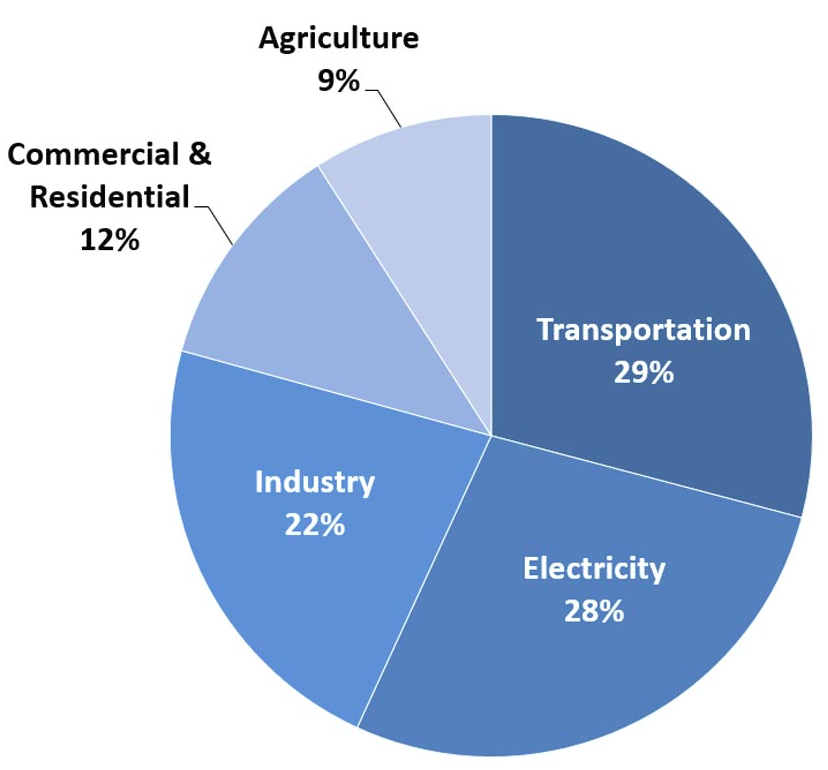
\includegraphics[height=5.0cm]{images/total-ghg-2017.png}
		\end{center}
		\caption{Total U.S. GHG Emissions by Economic Sector in 2017 \cite{us_epa_sources_2020}.}
	\end{figure}

	\column[t]{5cm}
	\\
	Illinois Climate Action Plan (iCAP):
	\begin{itemize}
		\item Main goal: carbon neutrality by 2050.
	\end{itemize}
	\vspace{0.75cm}
	Six target areas:
	\begin{itemize}
		\item Energy conservation.
		\item Energy generation, purchasing, and distribution.
		\item Transportation.
		\item Water and storm water.
		\item Waste and recycling.
		\item Agriculture, land use, and food.
	\end{itemize}
\end{columns}
\end{frame}

% Notes:
% Transportation and Electricity are the economic sectors that produced ...


\begin{frame}
\frametitle{Transportation}
\begin{columns}
	\column[t]{4.cm}
	\\
    Fuel Cell Electric Vehicles (FCEV):
	\begin{itemize}
		\item Address global warming concerns.
		\item Limitation on fossil fuel supply.
		\item Japan, Germany, and California.
		\item Champaign-Urbana.
	\end{itemize}

    \column[t]{6.cm}
	\begin{figure}[htbp!]
		\begin{center}
			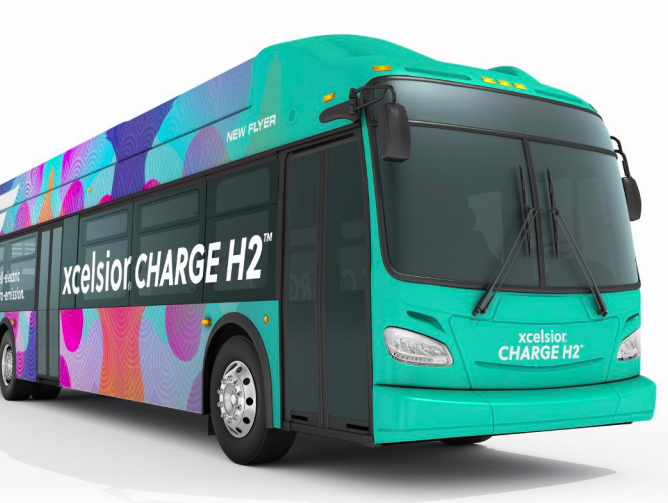
\includegraphics[height=5cm]{images/bus.png}
		\end{center}
		\caption{New Flyer fuel cell bus.}
	\end{figure}
\end{columns}
\end{frame}


\begin{frame}
\frametitle{Energy generation}
\begin{columns}
	\column[t]{4cm}
	\\
	Obvious solution:
	\begin{itemize}
		\item More renewables.
	\end{itemize}

    New problem:
	\begin{itemize}
		\item Duck curve.
		\item Demand ramps.
		\item Over-generation.
	\end{itemize}

    Consequences:
	\begin{itemize}
		\item Increase in dispatchable generation.
		\item Decrease in non-dispatchable generation.
	\end{itemize}

    \column[t]{6cm}
	\begin{figure}[htbp!]
		\begin{center}
			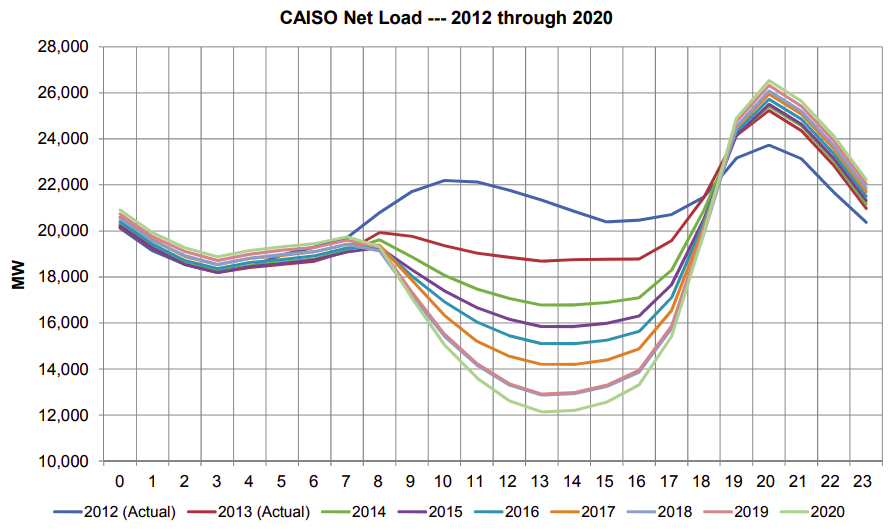
\includegraphics[height=4.0cm]{images/caiso-duck.png}
		\end{center}
		\caption{The duck curve.}
	\end{figure}
\end{columns}
\end{frame}


\begin{frame}
\frametitle{A possible solution}
    \textbf{Nuclear reactors and hydrogen:}
	\begin{itemize}
		\item Energy produced with no carbon emissions.
		\item Produce hydrogen as main/secondary product.
		\item Hydrogen as fuel for the FCEV.
		\item Hydrogen as electricity storage.
	\end{itemize}
	\centering
	\vspace{1cm}
	\textbf{Approach consistent with our goal of reducing carbon emissions!!}
\end{frame}


\begin{frame}
\frametitle{Microreactors}
\begin{columns}
	\column[t]{5cm}
	\begin{itemize}
		\item Several designs are under development in the US.
		\item Plug-and-play reactors.
		\item Remote commercial applications.
		\item Remote military bases.
	\end{itemize}
	\vspace{1cm}
	Features:
	\begin{itemize}
		\item Factory fabricated.
		\item Transportable.
		\item Self-regulating.
	\end{itemize}

    \column[t]{5cm}
	\begin{figure}[htbp!]
		\begin{center}
			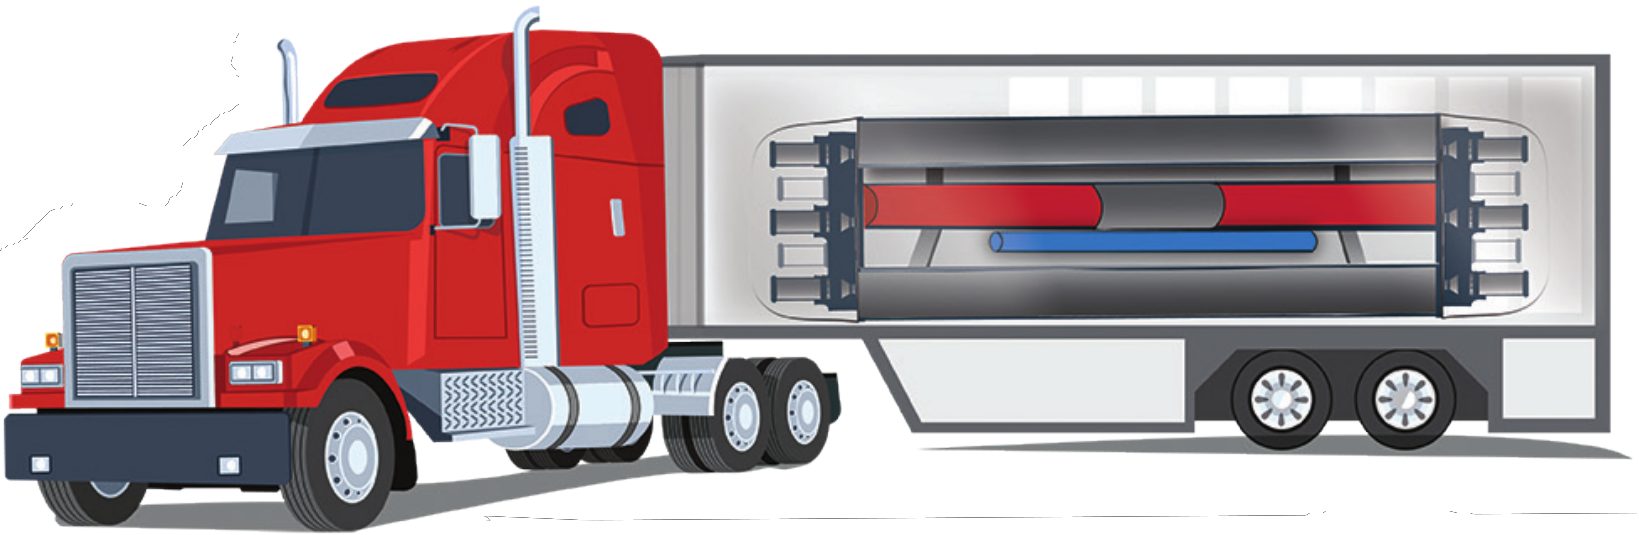
\includegraphics[width=5.2cm]{images/microreactor}
		\end{center}
		\caption{Microreactor design.}
	\end{figure}
\end{columns}
\end{frame}


\begin{frame}
\frametitle{Objectives}
\centering
    \begin{enumerate}
    	\item Replace use fossil fuels by CU MTD and UIUC fleets with hydrogen.
    	\item Supply the hydrogen with a or a series of microreactors.
    	\item Analyze the likelihood of the duck curve in Champaign-Urbana.
        \item Mitigate the duck curve negative effects.
	\end{enumerate}
\end{frame}

\section{Hydrogen Production}
\begin{frame}
\frametitle{Electrolysis}
\begin{columns}
    \column[t]{5cm}
	\begin{figure}[htbp!]
		\begin{center}
			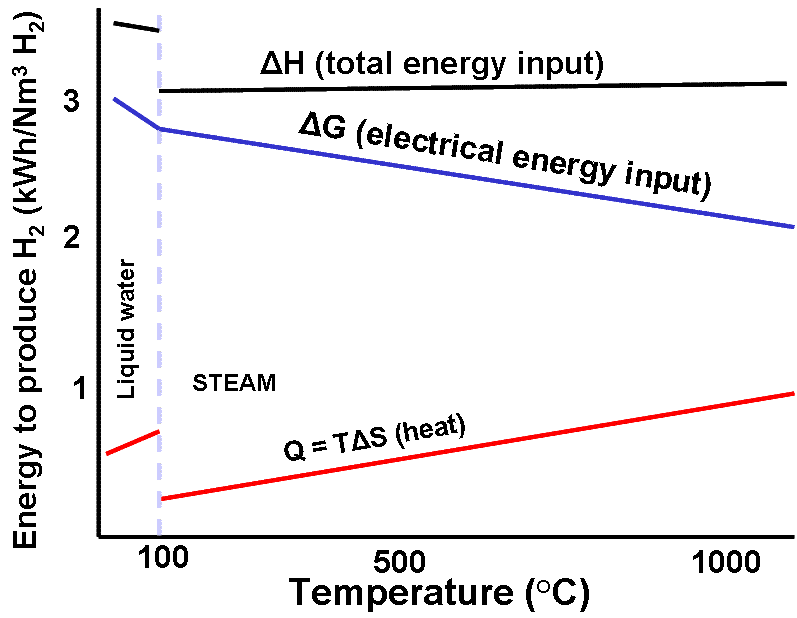
\includegraphics[height=4.0cm]{images/ele-curve.png}
		\end{center}
		\caption{Energy consumption of an ideal electrolysis process \cite{hi2h2_highly_2007}.}
	\end{figure}

	\column[t]{5cm}
	$\Delta$H: Required energy.
	\\
	$\Delta$G: Electrical energy.
	\\
	T$\Delta$S: Thermal energy. \vspace{0.7cm}

    In low temperature electrolysis (LTE), electricity provides the thermal energy.
    \\
    In high temperature electrolysis (HTE), heat source provides the thermal energy.
    \\
    HTE has the advantage of decreasing the electricity requirement.
    
\end{columns}
\end{frame}


\begin{frame}
\frametitle{Sulfur-Iodine}
\begin{columns}
    \column[t]{5cm}
   	\begin{figure}[htbp!]
		\begin{center}
			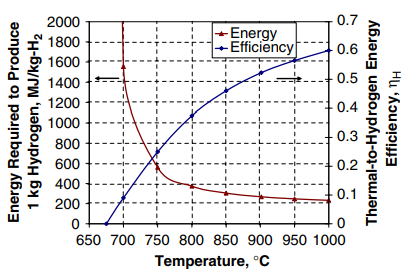
\includegraphics[height=4.0cm]{images/si-energy.png}
		\end{center}
		\caption{Sulfur-Iodine thermochemical cycle.}
 	\end{figure}

 	\column[t]{5cm}
 	\begin{itemize}
 		\item 3 different reactions: Sulfuric acid decomposition, Bunsen reaction, and hydrogen iodide decomposition.
 		\item Input: H$_2$O.
 		\item Output: H$_2$ $\&$ O$_2$. 
 		\item Does not require electricity.
 		\item Need of a high temperature source.
 	\end{itemize}
\end{columns}
\end{frame}


\begin{frame}
\frametitle{Co-generation}
\begin{columns}
    \column[t]{6.5cm}
   	\begin{figure}[htbp!]
		\begin{center}
			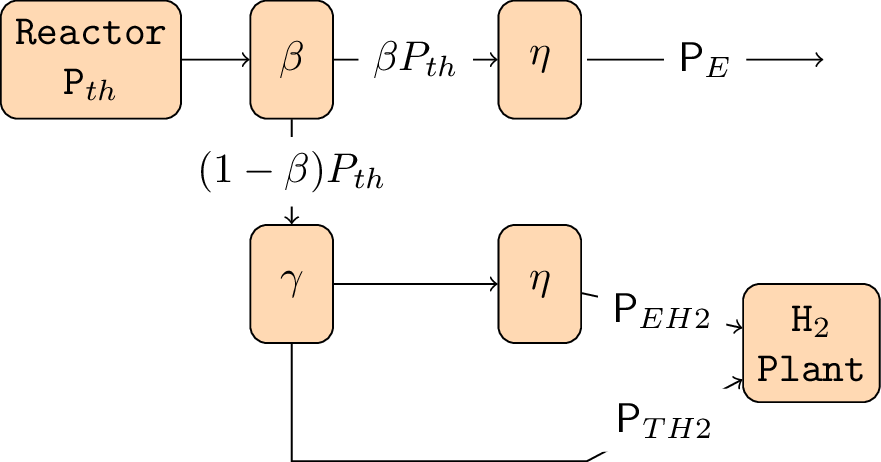
\includegraphics[height=3.6cm]{images/hte-figure0.png}
		\end{center}
		\caption{Reactor coupled to hydrogen plant diagram.}
 	\end{figure}

 	\column[t]{3.5cm}
 	$\beta$: power fraction that is converted into electricity.
 	\\
    $\beta$ = 1: no hydrogen is produced.
    \\
 	$\beta$ = 0: no electricity is produced. \vspace{0.6cm}

 	LTE:
 	\begin{itemize}
 		\item $\gamma$=1. P$_{TH2}$ = 0.
 	\end{itemize}

 	HTE:
 	\begin{itemize}
 		\item 0 $< \gamma <$ 1.
 	\end{itemize}

    SI:
 	\begin{itemize}
 		\item $\gamma$=0. P$_{EH2}$ = 0.
 	\end{itemize}


\end{columns}
\end{frame}

\section{Results}
\begin{frame}
\frametitle{Transportation: fuel demand}
\begin{columns}
    \column[t]{5cm}
	\begin{figure}[htbp!]
		\begin{center}
			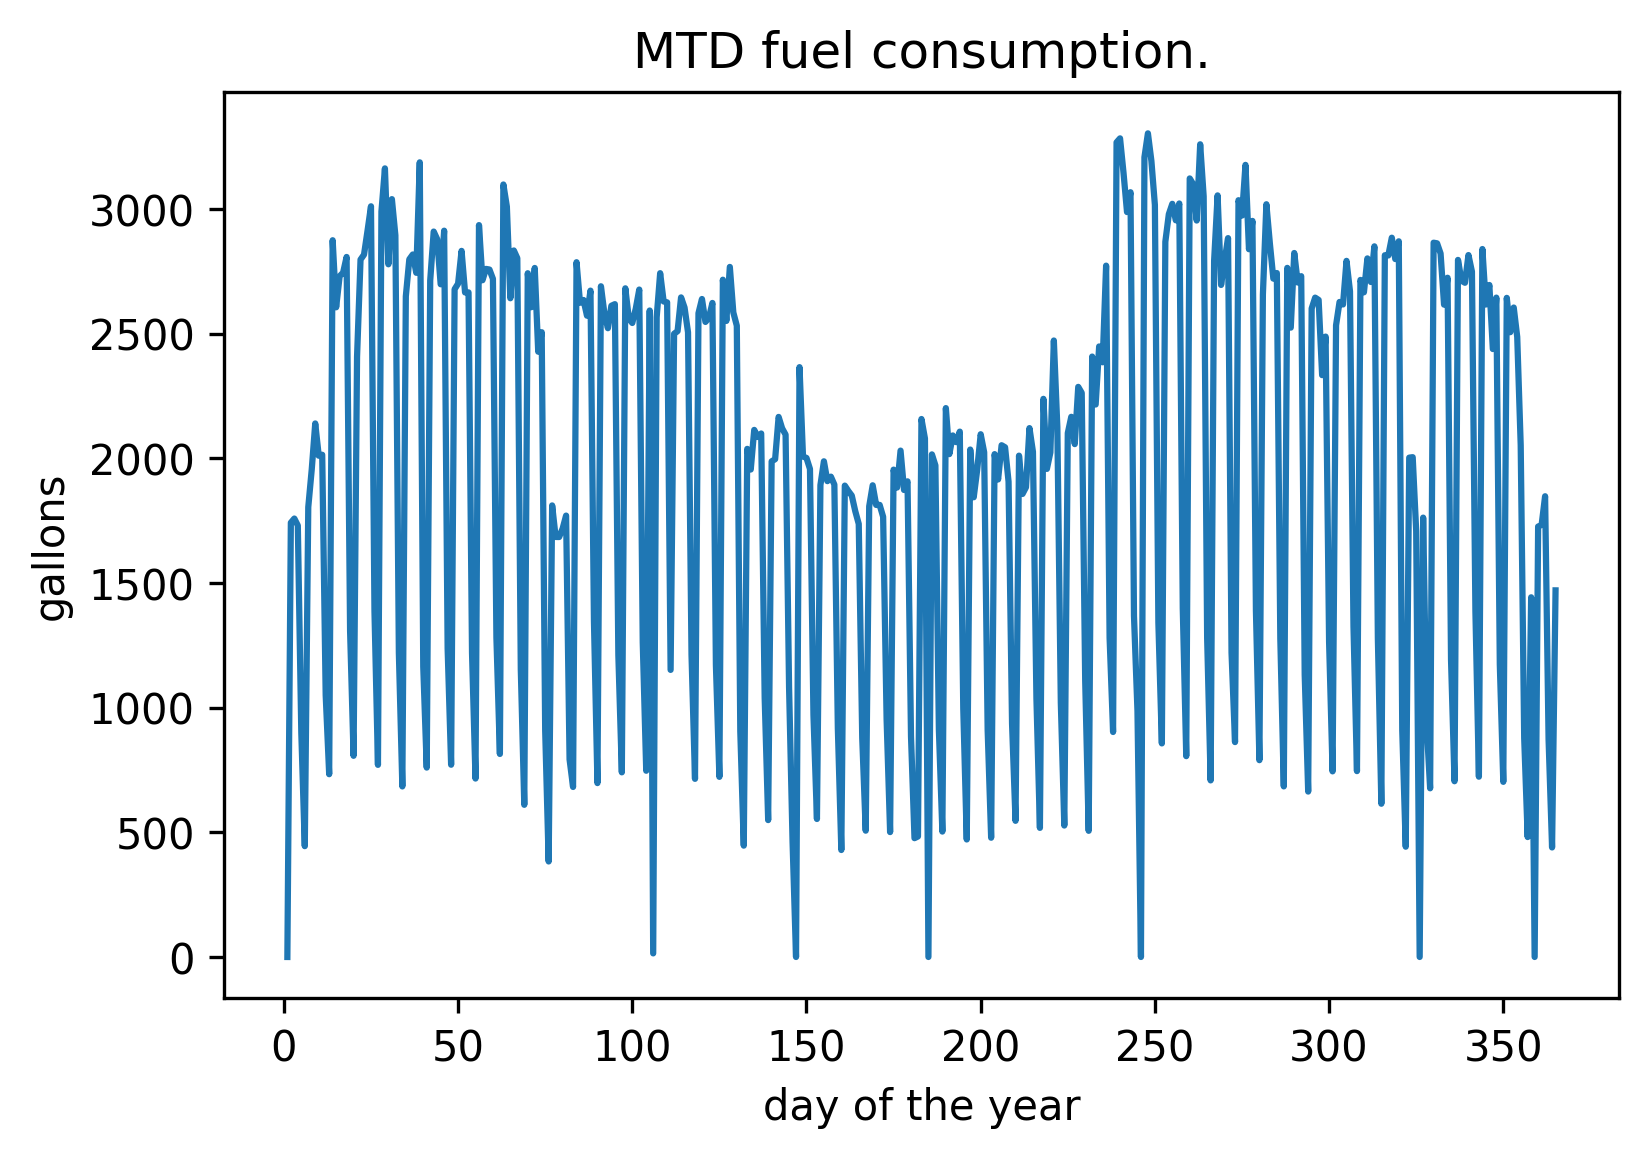
\includegraphics[height=3.5cm]{images/mtd2}
		\end{center}
		\caption{MTD fuel consumption.}
	\end{figure}

	\column[t]{5cm}
	\begin{figure}[htbp!]
		\begin{center}
			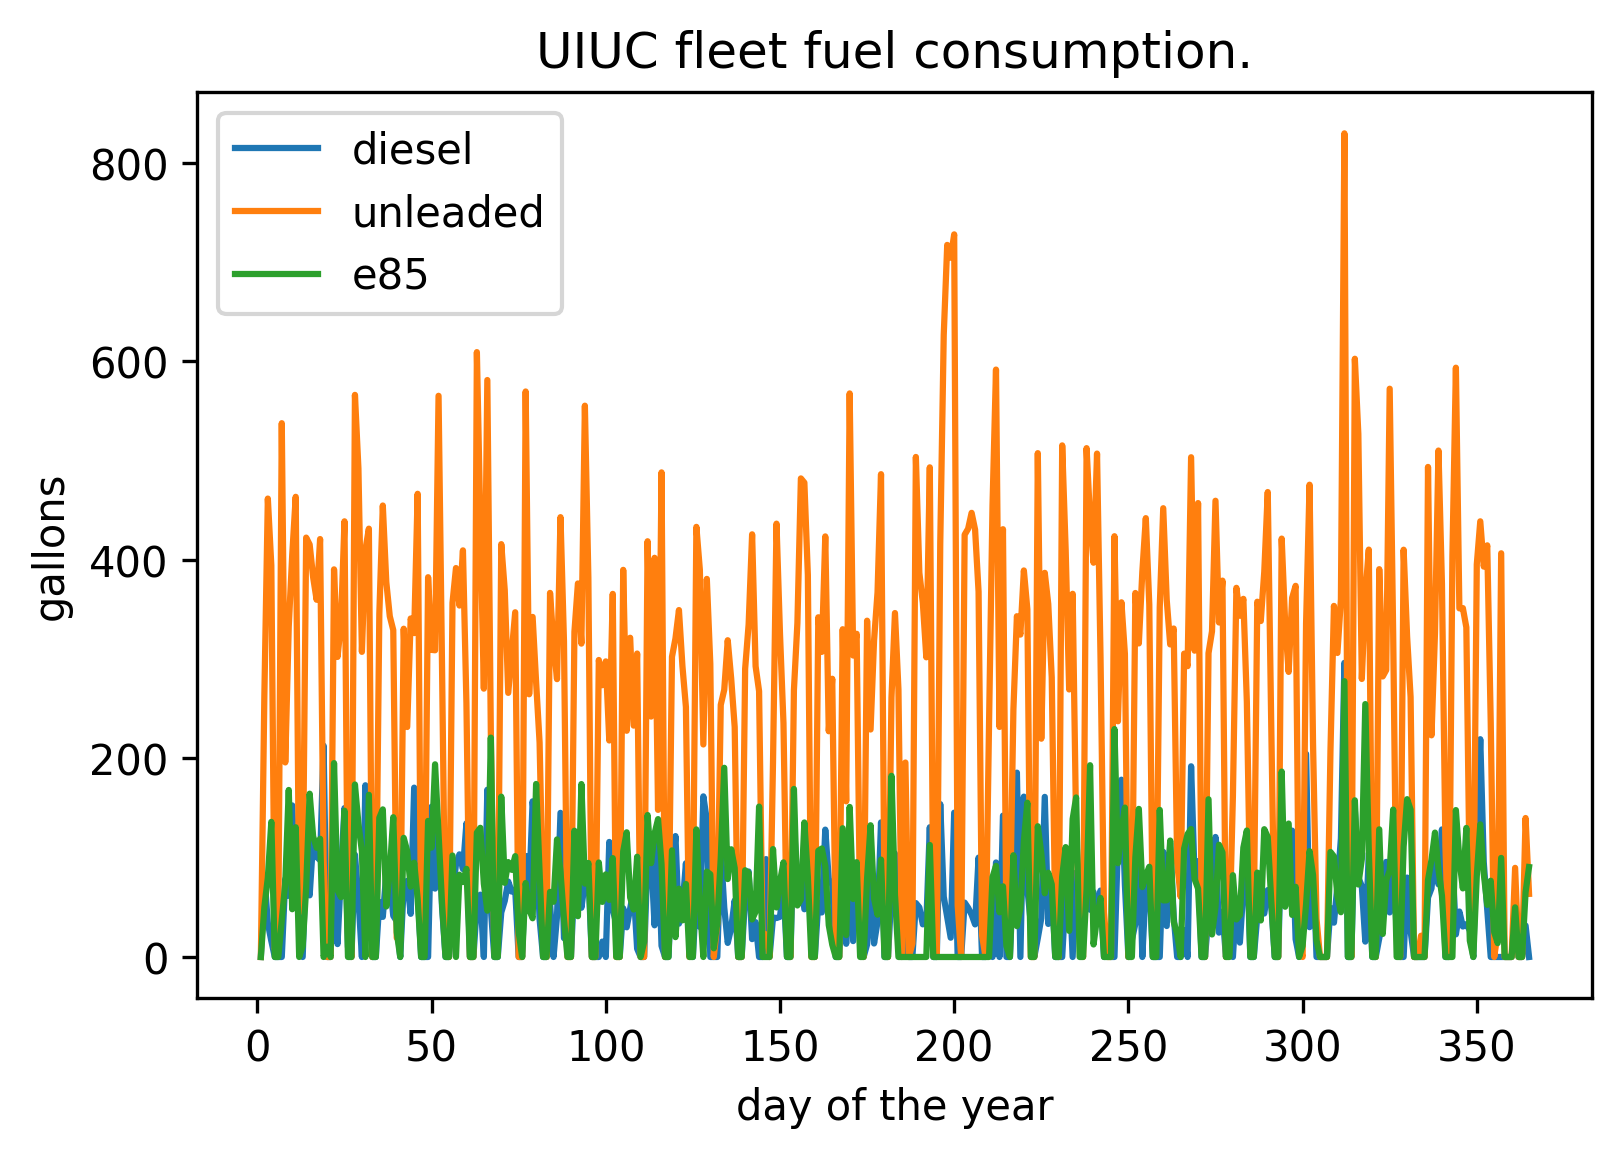
\includegraphics[height=3.5cm]{images/uiuc}
		\end{center}
		\caption{UIUC fleet fuel consumption.}
	\end{figure}
\end{columns}
\end{frame}


\begin{frame}
\frametitle{Transportation: fuel demand}
\begin{columns}
    \column[t]{5cm}
	\begin{table}[!htb]
		\centering
	    \caption{GGE, DGE, and E85GE.}
		\begin{tabular}{l|l}
		\hline
		                 & Hydrogen \\ \hline
		GGE              & 1 kg     \\
		DGE              & 1.13 kg  \\
		E85GE            & 0.78 kg  \\ \hline
        \end{tabular}
	\end{table}

	\begin{table}[!htb]
		\centering
	    \caption{Hydrogen requirements.}
		\begin{tabular}{l|l}
		\hline
		Total [tonnes/year]  & 943      \\
		Average [kg/day] 	 & 2584     \\
		Average [kg/h] 		 & 108      \\
		Maximum in one day   & 4440 kg  \\ \hline
        \end{tabular}
	\end{table}

	\column[t]{5cm}
	\begin{figure}[htbp!]
		\begin{center}
			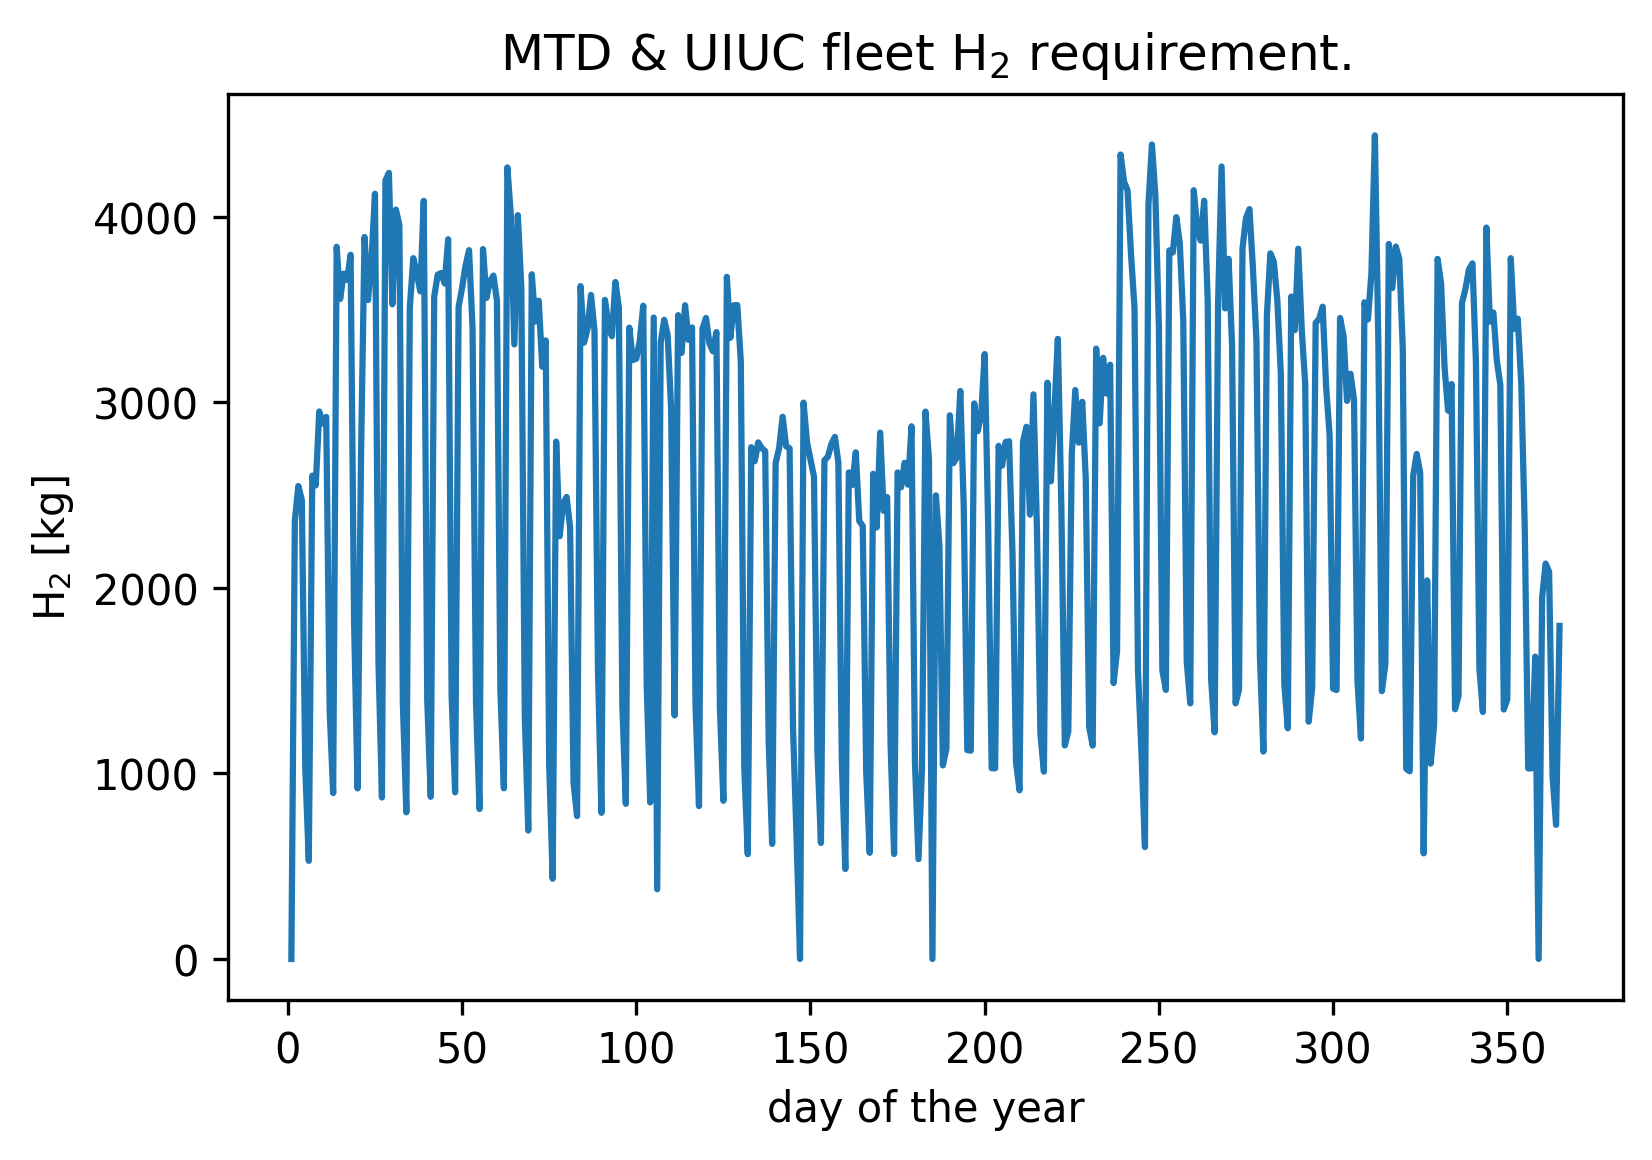
\includegraphics[height=3.5cm]{images/hydro-fleet}
		\end{center}
		\caption{MTD and UIUC fleets hydrogen requirement.}
	\end{figure}

\end{columns}
\end{frame}


\begin{frame}
\frametitle{Transportation: fuel demand}
\begin{columns}
    \column[t]{4.5cm}
	\begin{table}[!htb]
		\centering
	    \caption{Microreactor designs.}
		\begin{tabular}{l|ll}
		\hline
		Reactor      & P[MW$_{th}$] & T$_o$[$^\circ$C]\\ \hline
		MMR          & 15         & 640             \\
		eVinci       & 5          & 650             \\
		ST-OTTO      & 30         & 750             \\
		U-battery    & 10         & 750             \\
		Starcore     & 36         & 850             \\ \hline
        \end{tabular}
	\end{table}

	\column[t]{5.5cm}
	\begin{figure}[htbp!]
		\begin{center}
			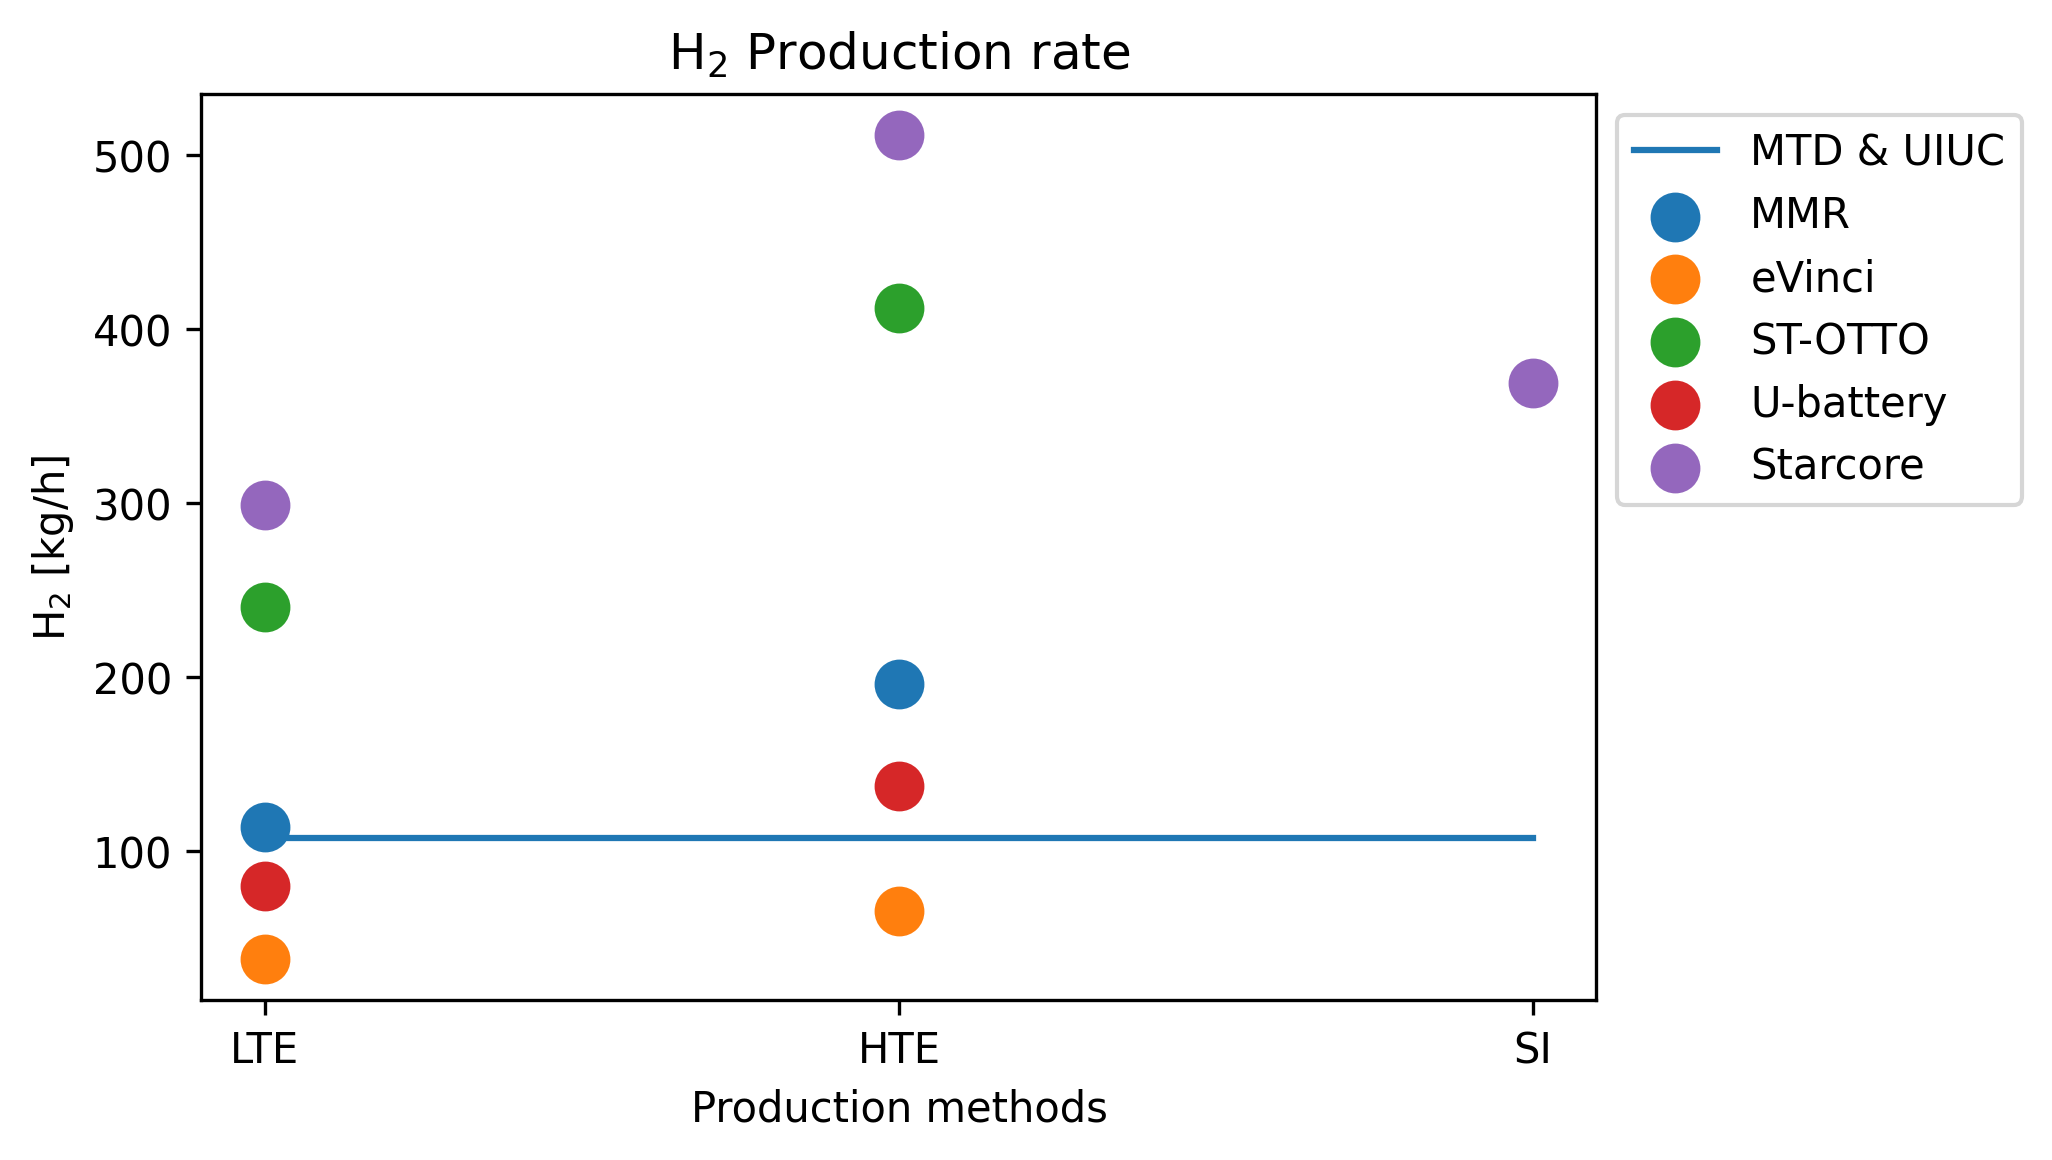
\includegraphics[height=3.5cm]{images/reactors-by-hour1}
		\end{center}
		\caption{Hydrogen production rate by different microreactor designs.}
	\end{figure}

\end{columns}
\end{frame}


\begin{frame}
\frametitle{Energy generation}
\begin{columns}
    \column[t]{5cm}
	\begin{figure}[htbp!]
		\begin{center}
			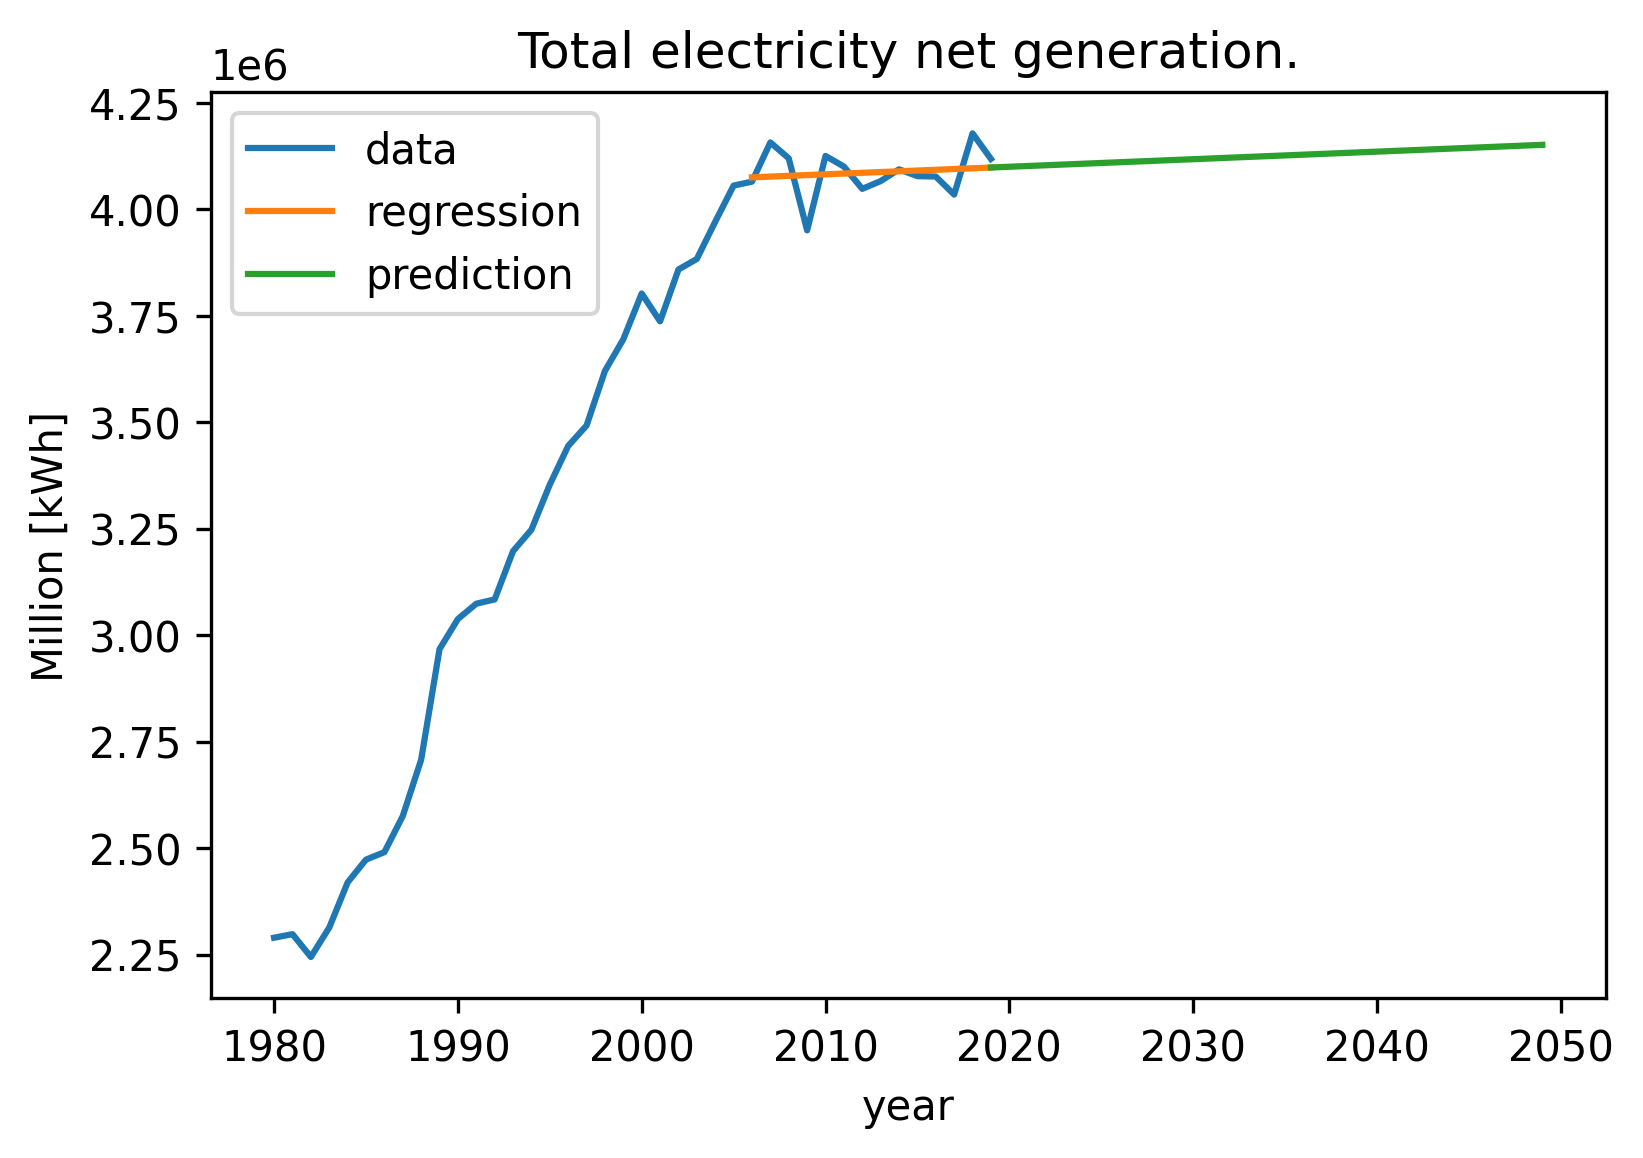
\includegraphics[height=3.3cm]{images/us-prediction1}
		\end{center}
		\caption{Prediction on the total electricity generation in the US for 2050.}
	\end{figure}

    \column[t]{5cm}
	\begin{figure}[htbp!]
		\begin{center}
			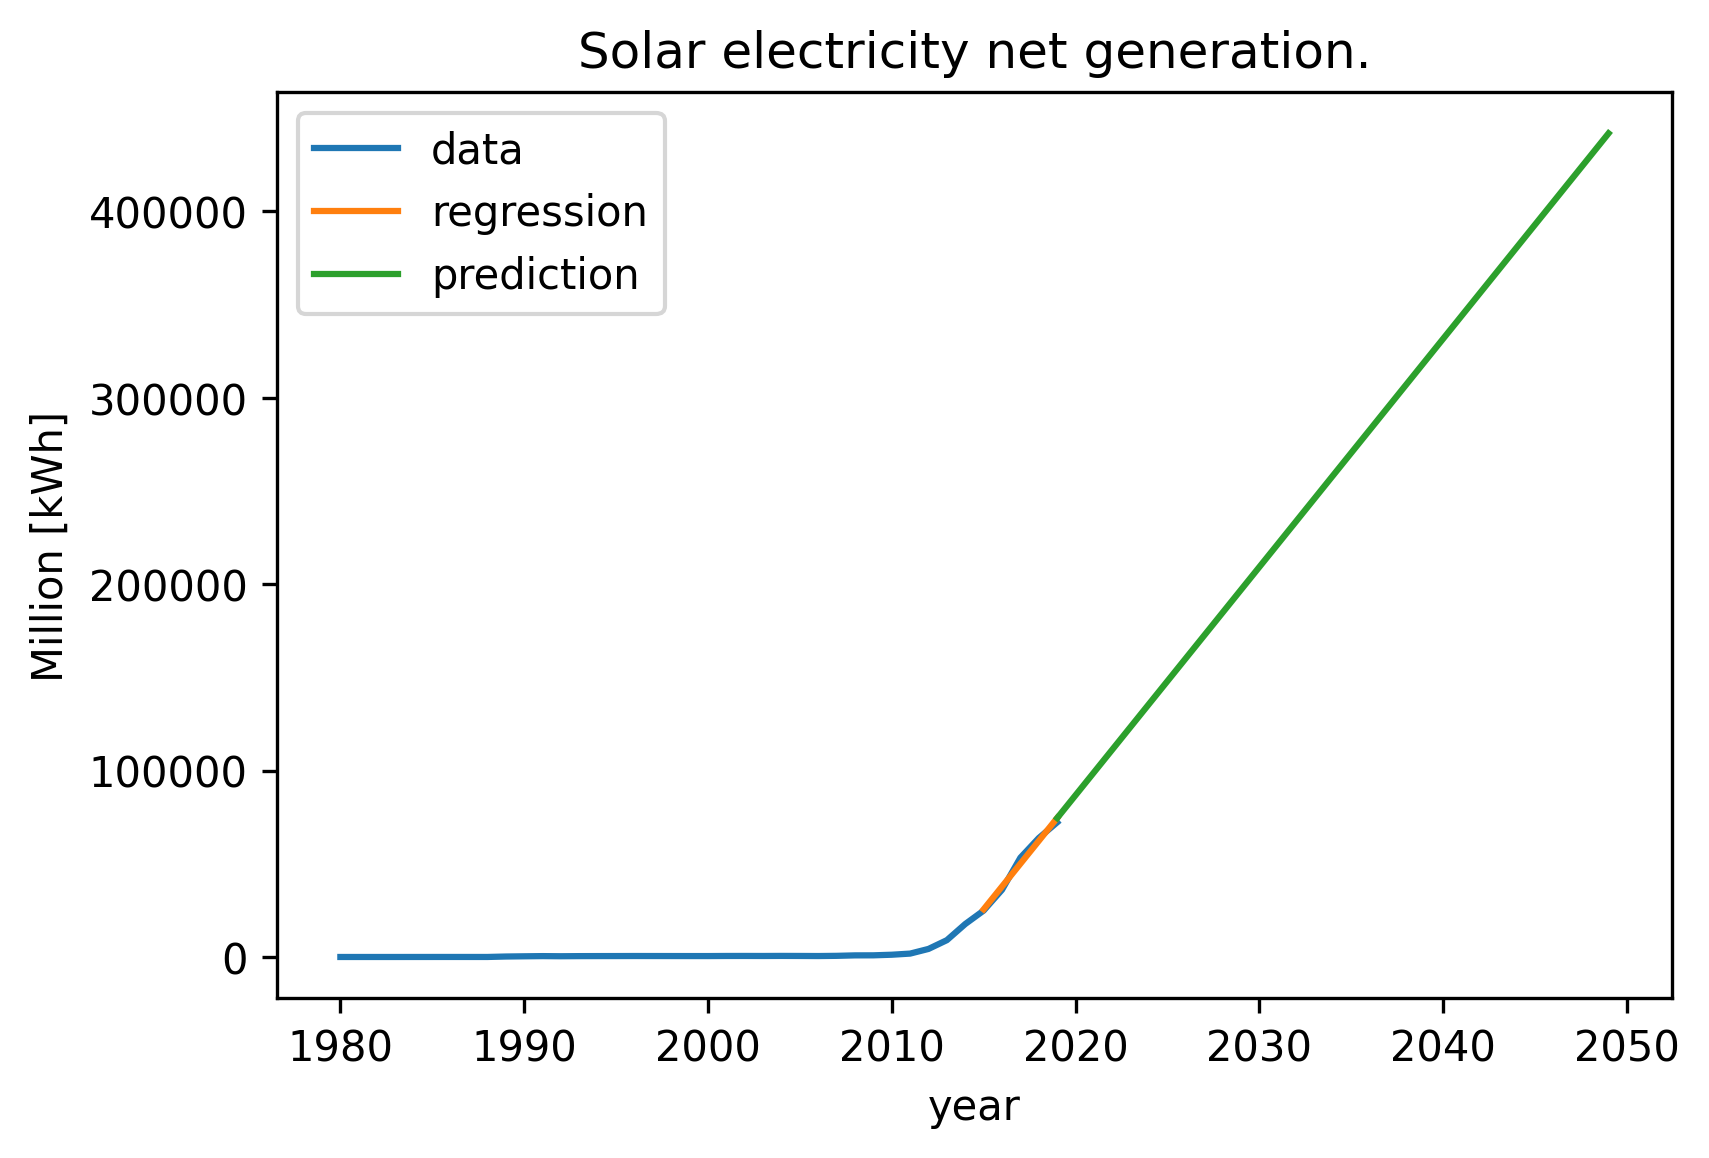
\includegraphics[height=3.3cm]{images/us-prediction2}
		\end{center}
		\caption{Prediction on the solar electricity generation in the US for 2050.}
	\end{figure}
\end{columns}
\end{frame}


\begin{frame}
\frametitle{Duck curve}
\begin{columns}
    \column[t]{4.5cm}
	\begin{figure}[htbp!]
		\begin{center}
			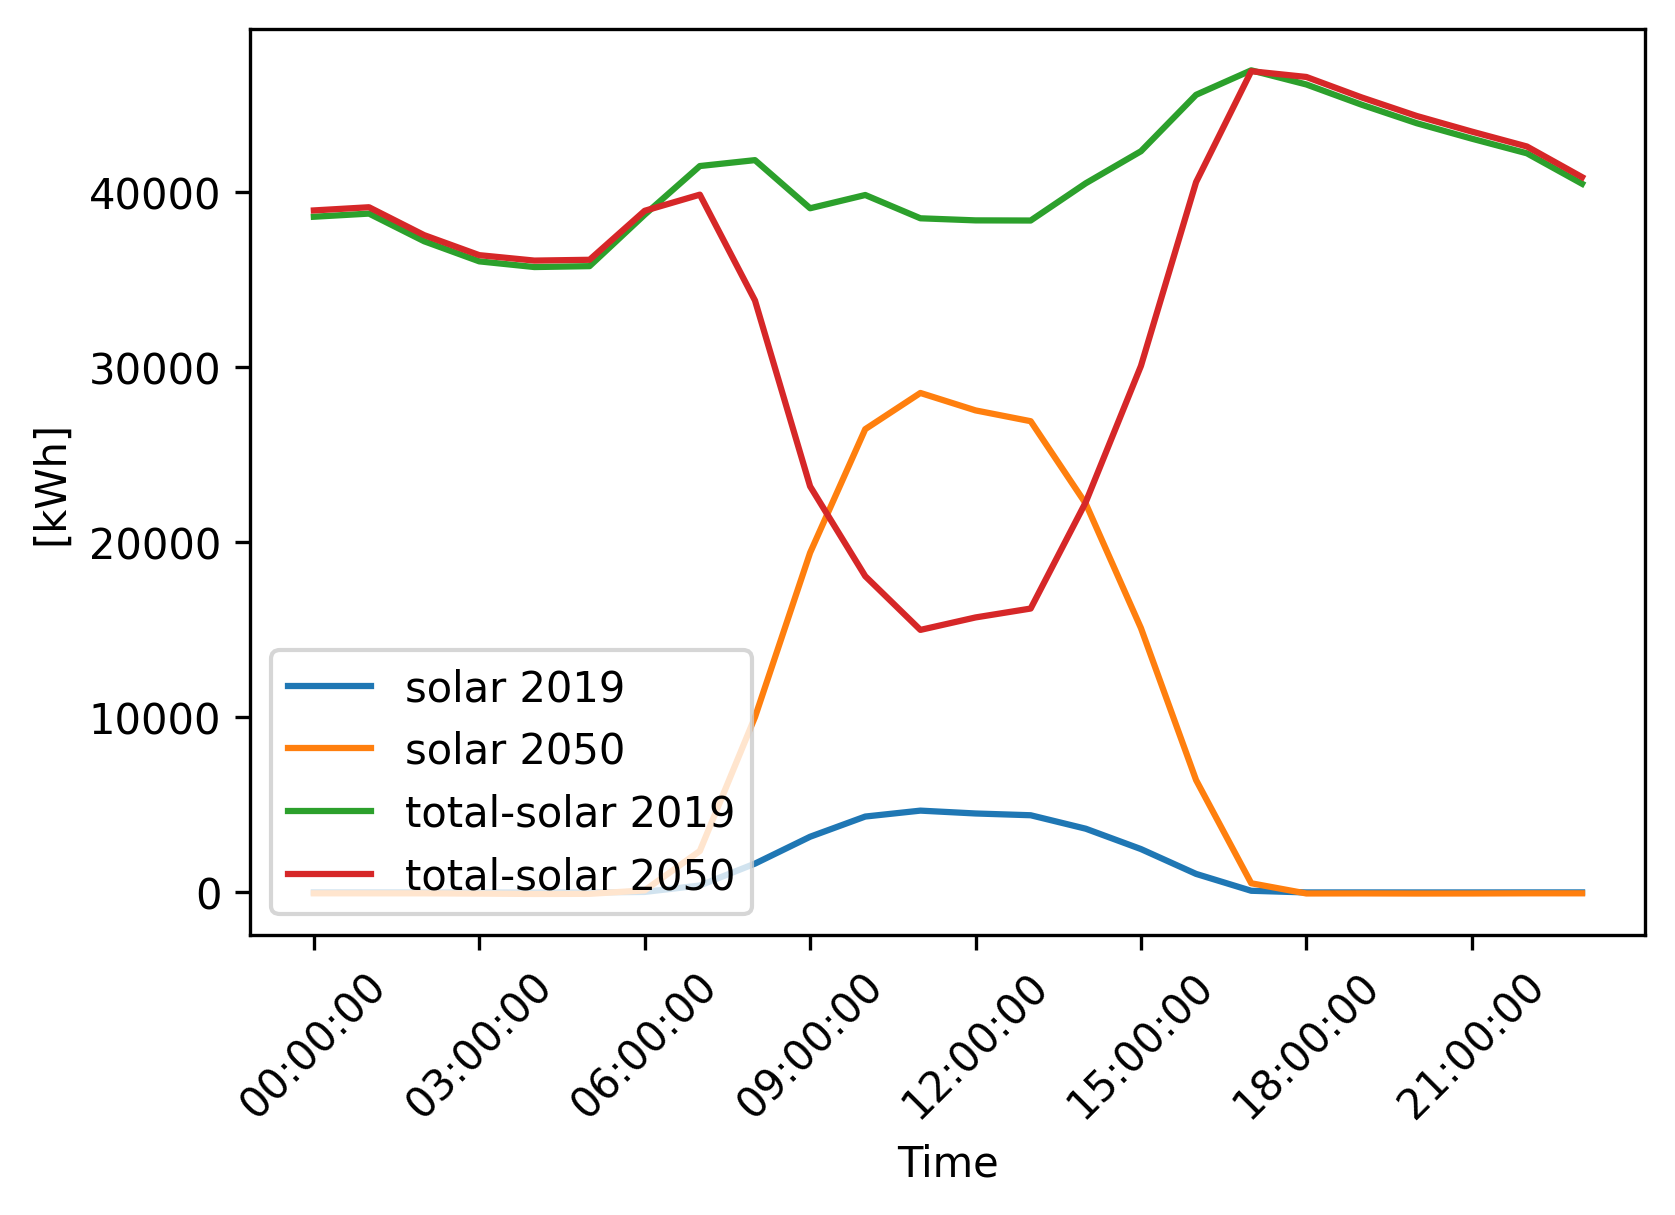
\includegraphics[height=4.0cm]{images/uiuc-duck}
		\end{center}
		\caption{Prediction on UIUC's demand for 2050.}
	\end{figure}

    \column[t]{5.5cm}
    \begin{itemize}
 		\item Spring: solar production is higher, total demand is low.
 		\item Solar generation peaked on April 4, 2019.
 		\item Peak demand is 46.9 MWh at 5 P.M.
 		\item Lowest demand is 15 MWh at 11 A.M.
 		\item Requires an installed capacity of 31.9 MW of dispatchable sources.
 	\end{itemize}

\end{columns}
\end{frame}


\begin{frame}
\frametitle{Duck curve}
\begin{columns}
    \column[t]{5.5cm}
	\begin{figure}[htbp!]
		\begin{center}
			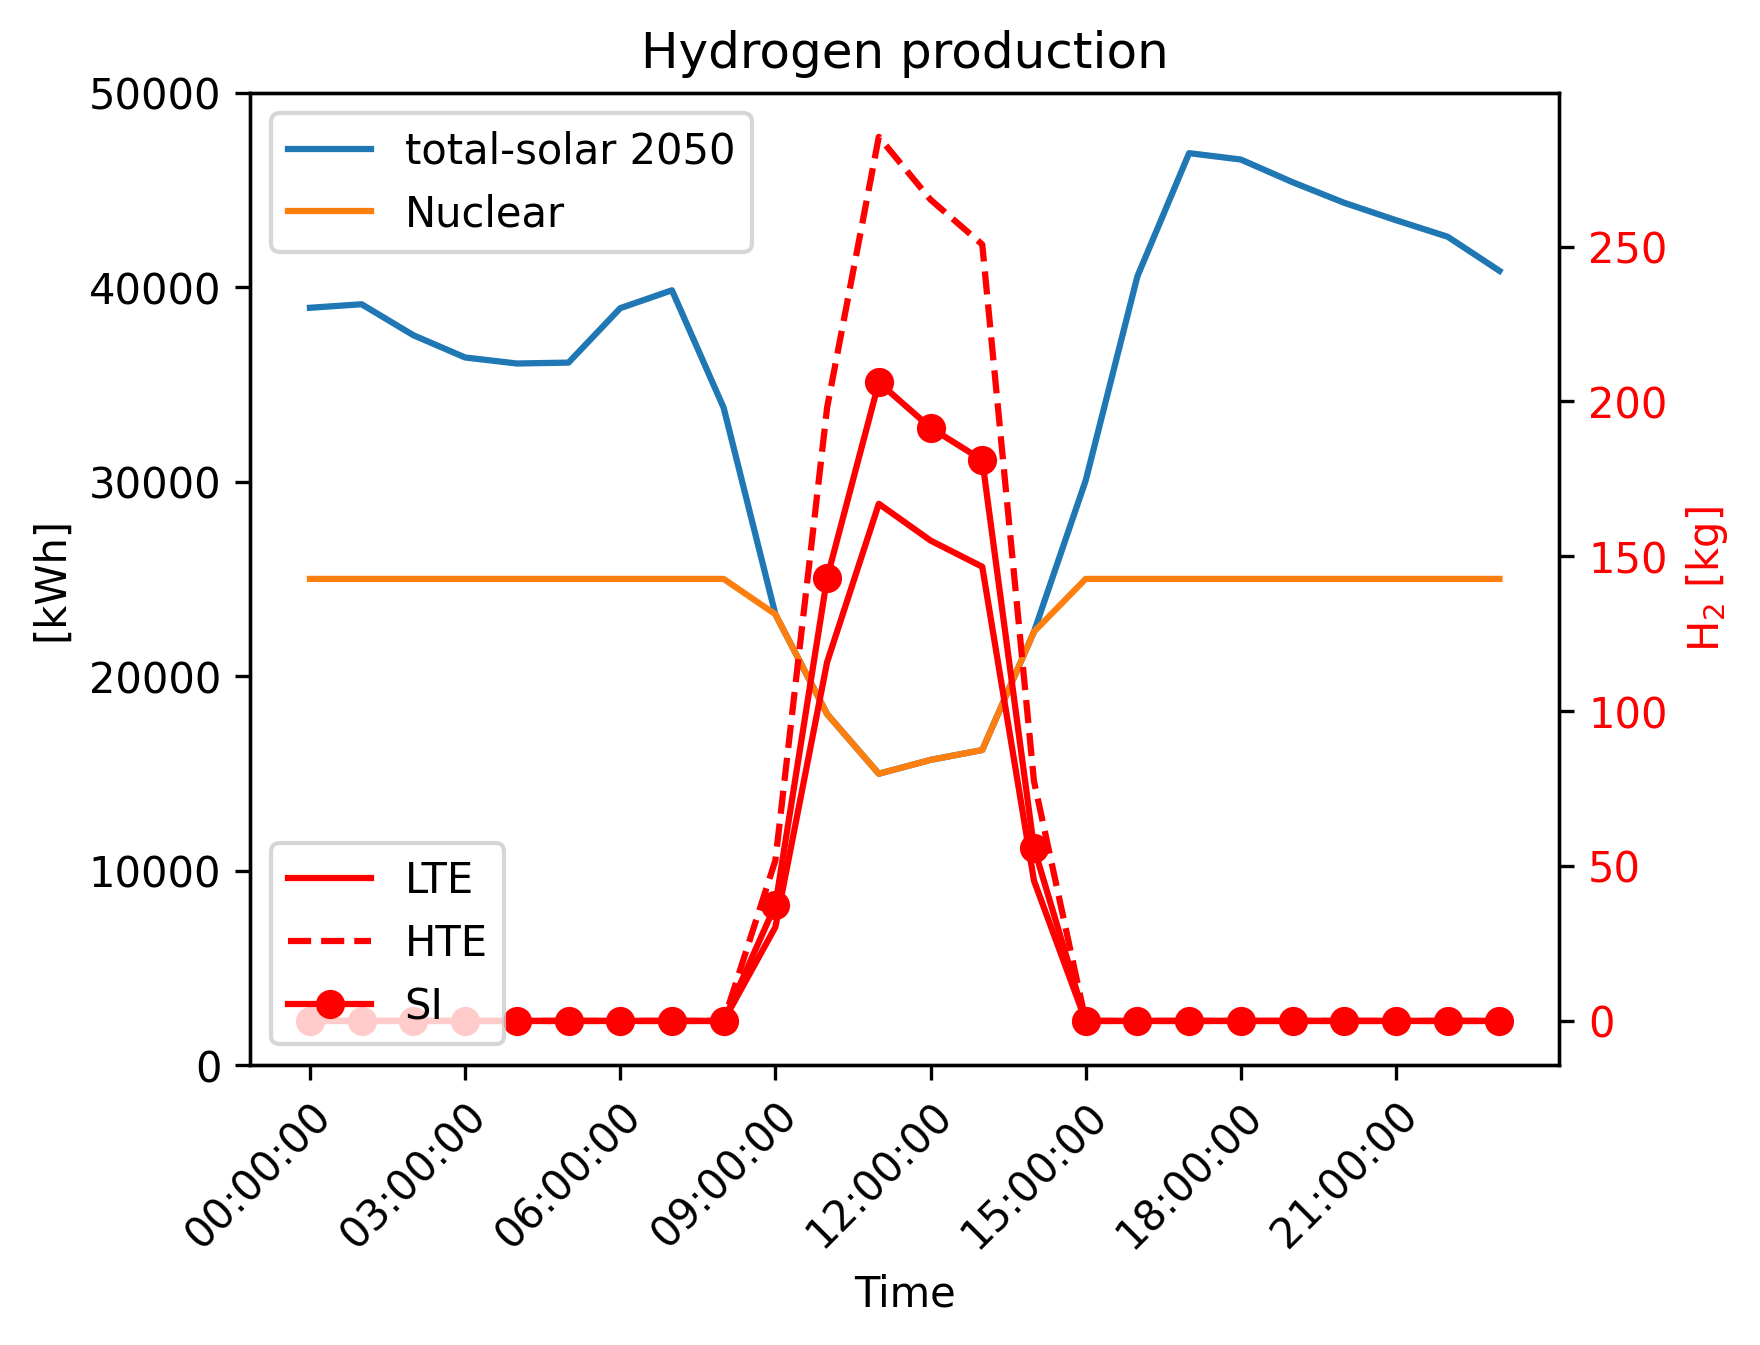
\includegraphics[height=4.4cm]{images/uiuc-hydro2B}
		\end{center}
		\caption{Hydrogen production with the excess of energy.}
	\end{figure}

    \column[t]{4.5cm}
    25 MWe reactor. \vspace{0.2cm}

    LTE:
    \begin{itemize}
 		\item $\eta$=33$\%$.
 		\item 660 kg-H$_2$.
 	\end{itemize}

    HTE:
    \begin{itemize}
 		\item HTGR.
 		\item T$_o$ = 850$^\circ$C.
 		\item $\eta$=49.8$\%$
 		\item 1129 kg-H$_2$.
 	\end{itemize}

    SI:
    \begin{itemize}
 		\item HTGR.
 		\item T$_o$ = 850$^\circ$C.
 		\item $\eta$=49.8$\%$
 		\item 815 kg-H$_2$.
 	\end{itemize}

\end{columns}
\end{frame}

\begin{frame}
\frametitle{Hydrogen for energy storage}
\begin{columns}
    \column[t]{6.5cm}
	\begin{figure}[htbp!]
		\begin{center}
			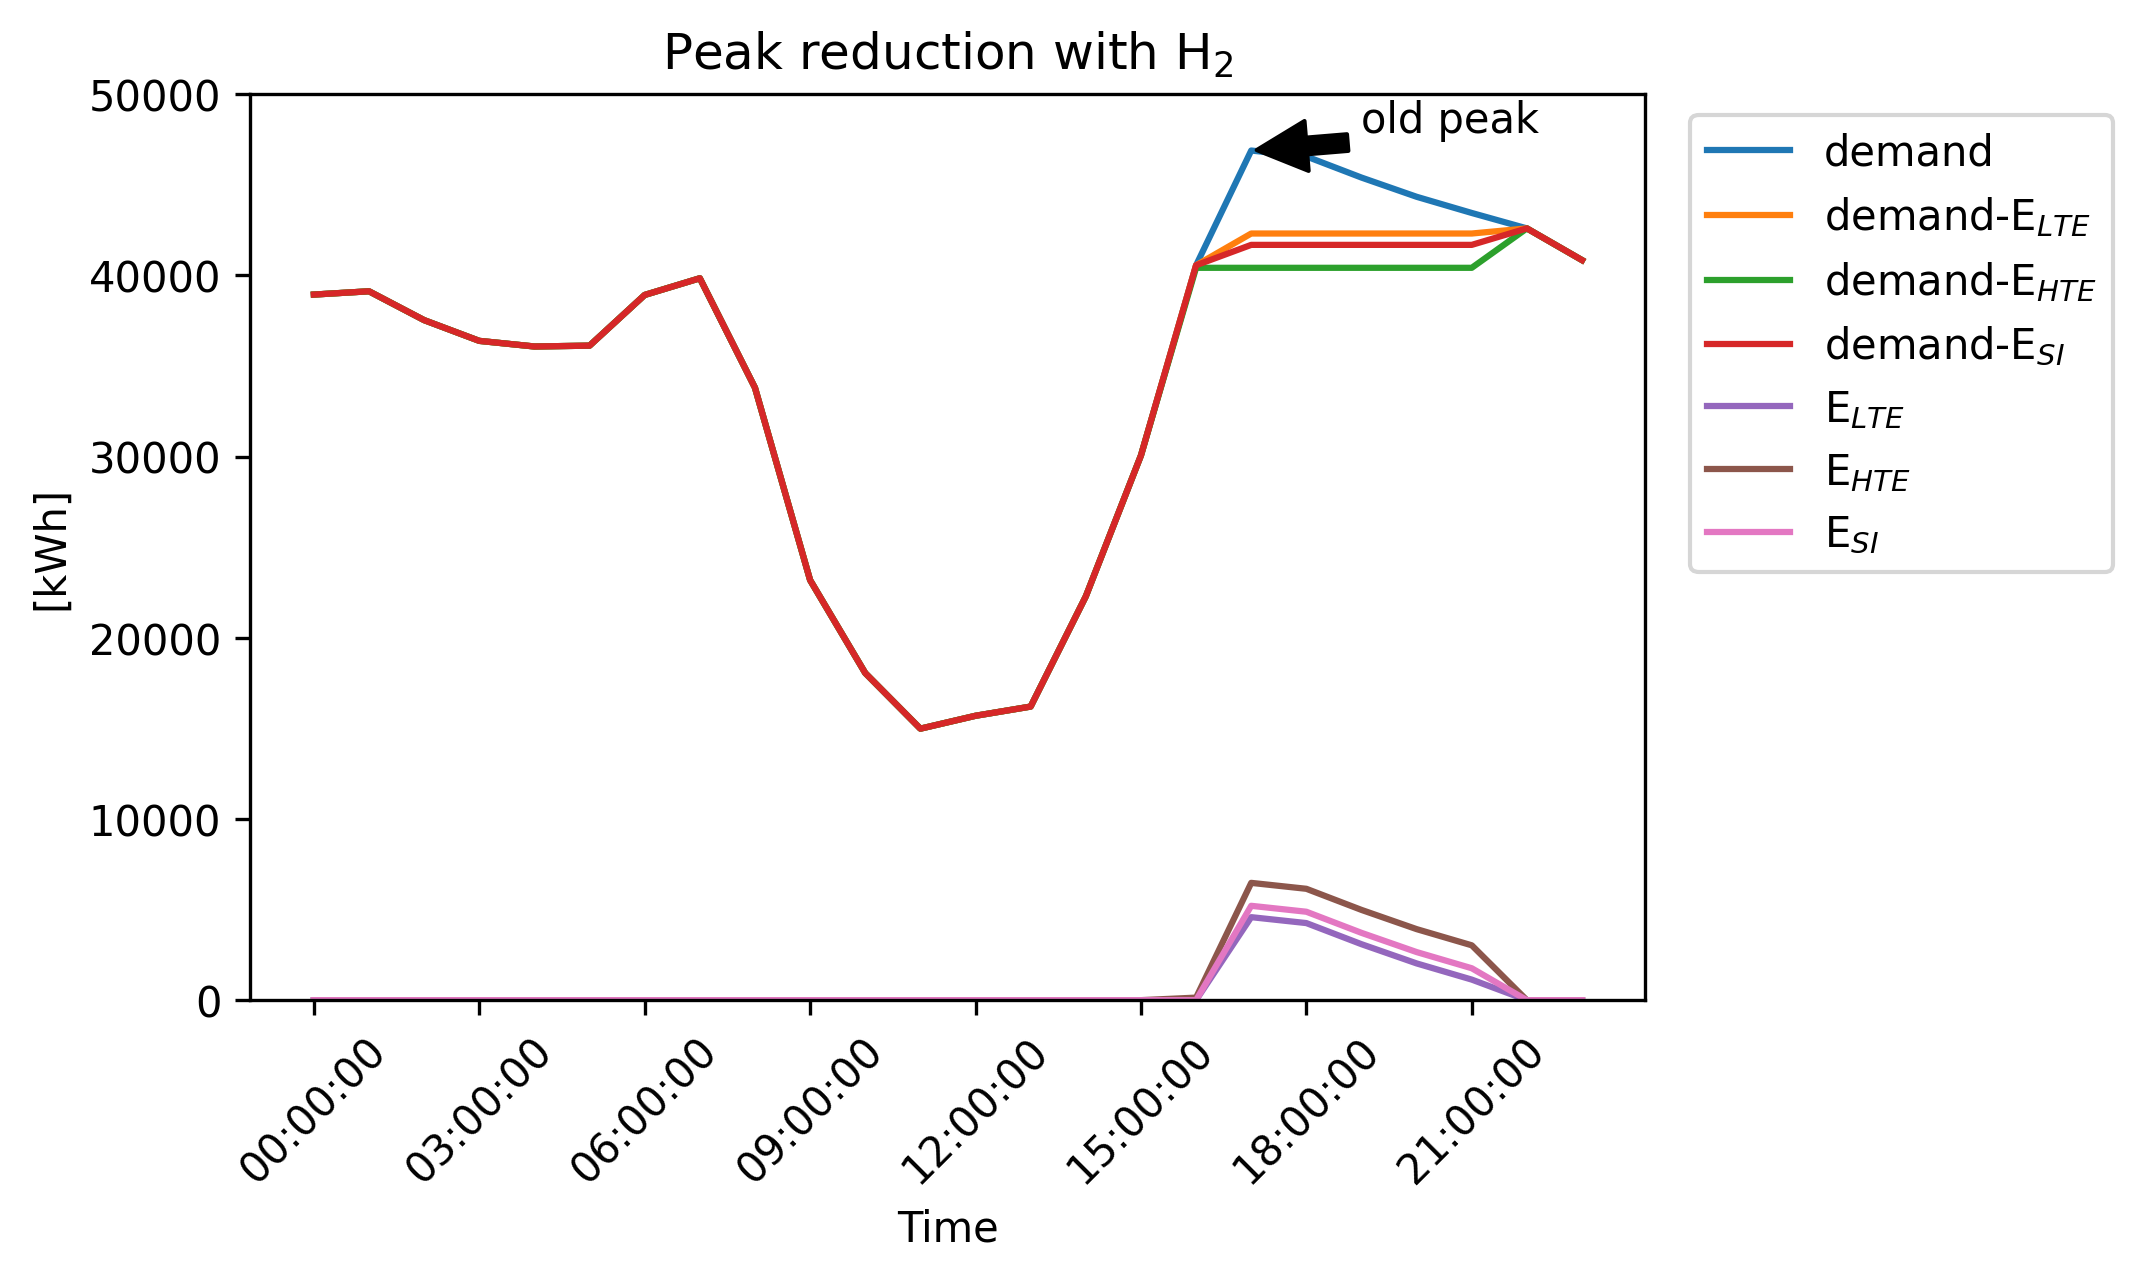
\includegraphics[height=4.2cm]{images/uiuc-hydro3B}
		\end{center}
		\caption{Peak reduction by using the produced H$_2$.}
	\end{figure}

    \column[t]{4.5cm}
    \\
    LTE:
    \begin{itemize}
 		\item 15.9 MWh.
 		\item New peak: 41.9 MWh
 		\item Peak reduction: 5 MWh
 	\end{itemize}

    HTE:
    \begin{itemize}
		\item 27.1 MWh.
		\item New peak: 40.0 MWh
        \item Peak reduction: 6.9 MWh
 	\end{itemize}

    SI:
    \begin{itemize}
		\item 19.6 MWh.
		\item New peak: 41.3 MWh
        \item Peak reduction: 5.6 MWh
 	\end{itemize}

\end{columns}
\end{frame}

% \section{Future studies}
% \input{future}

\section{Conclusion}
\begin{frame}
\frametitle{Conclusions}

\begin{itemize}
	\item The University of Illinois is actively working to reduce GHG emissions on its campus. 
	\item A few microreactor designs would be able to produce enough hydrogen to meet MTD and UIUC fleet fuel demand.
	\item An excessive integration of PV to UIUC grid make the duck curve phenomenon likely to occur.
	\item Nuclear energy and hydrogen production proposes an approach to mitigate the negative implications of the duck curve.
	\item Hydrogen introduces a way to store energy that reduces the reliance on dispatchable sources.

\end{itemize}
\end{frame}


\begin{frame}
\frametitle{Acknowledgement}

This work is supported the NRC Faculty Development Program.
\\
I would like to thank Sam Dotson (UIUC), Beth Brunk (MTD), and Pete Varney (UIUC) for their contributions to the development of this project.

\end{frame}

\begin{frame}[allowframebreaks]
  \frametitle{References}
  \bibliographystyle{plain}
  {\footnotesize \bibliography{bibliography.bib} }
\end{frame}

\end{document}
